\documentclass[a4paper]{article}
\usepackage[utf8]{inputenc}
\usepackage{graphicx}
\graphicspath{ {../data/} }
\usepackage[polish]{babel}
\usepackage[T1]{fontenc}
\usepackage{indentfirst}
\usepackage{amsmath, amsfonts}
\usepackage[nofoot,hdivide={2cm,*,2cm},vdivide={2cm,*,2cm}]{geometry}
\frenchspacing
\pagestyle{empty}

\author{Franciszek Zdobylak}
\title{\Huge{\bf{Gra w Statki}}\\
				\normalsize Instrukcja obsługi}

\begin{document}
\maketitle

\section{Wymagania}
\begin{itemize}
    \item Kompilator języka C (gcc)
    \item Program make
    \item Biblioteka GTK 3.0 oraz wszystkie biblioteki potrzebne przez nią
\end{itemize}

\section{Kompilowanie}
Aby móc korzystać z gry należy najpierw ją skompilować przy pomocy polecenia \texttt{make}.

\section{Uruchamianie}
Aby uruchomić grę należy wpisać w terminalu \texttt{./battleships N} gdzie \texttt{N} to nazwa użytkownika
(tj. A lub B). Aby program działał poprawnie obie kopie programu muszą być uruchomione.

\section{Obsługa Gry}
W oknie gry widoczne są plansze graczy (po lewej gracza po prawej przeciwnika). Grę rozpoczyna gracz A.

Gracz może wybierać pole, w które chce strzelić klikając na nie. Aby wykonać strzał musi trwać tura gracza,
inaczej zostanie wyświetlona informacja "Nie Twoja tura".

Status pola wyświetlany jest poprzez odpowiednią grafikę:
\begin{itemize}
    \item[$\bullet$] 
\includegraphics[width=1cm, height=1cm]{water.png} - pudło (na planszy przeciwnika)/ wolna przestrzeń (na planszy gracza)
    \item[$\bullet$] 
\includegraphics[width=1cm, height=1cm]{ship.png} - trafiony (na planszy przeciwnika)/ statek (na planszy gracza)
    \item[$\bullet$] 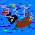
\includegraphics[width=1cm, height=1cm]{sunk.png} - zatopiony (na planszy przeciwnika)/ trafionu lub zatopiony (na planszy gracza)
    \item[$\bullet$] 
\includegraphics[width=1cm, height=1cm]{cloud.png} - nieznane pole (tylko na planszy przeciwnika)
\end{itemize}

Po prawej stronie plansz znajdują się statystyki gry oraz panel innych opcji dostępnych w grze.


\section{Tworzenie własnej planszy}
Aby stworzyć własną planszę należy kliknąć przycisk "Stwórz Planszę". Zostanie wtedy wyświetlone okno tworzenia planszy.
Można to zrobić jedynie wtedy gdy gra się jeszcze nie rozpoczęła.

Na samej górze okna wyświetla się krótka instrukcja jak to zrobić oraz liczba statków które zostały do rozmieszczenia na planszy.

Poniżej znajduje się panel wyboru statku (wybór orientacji oraz długości statku).

W centralnej części okna znajduje się plansza do rozmieszczania statkow. Statki umieszcza się poprzez kliknięcie w pole,
na którym ma się zaczynać statek. Jeśli statku nie można postawić na danym miejscu, (kolidowałby z innym, wychodził poza planszę
lub limit statków danej długości się wyczerpał) statek nie zostanie położony oraz wyświetli się stosowny komunikat.

Na samym dole znajduje sie przycisk do zatwierdzenia planszy (zostanie to zrobione jedynie wtedy gdy plansza jest poprawna,
tzn. wszystkie statki zostały rozmieszczone) oraz anulowania.

\section{Uwagi}
Aby program poprawnie działał należy nie wygkonywać żadnych czynności jeśli widzimy, że program jest w trakcie przetwarzania czegoś
(np. podczas odsłaniania planszy przeciwnika na koniec gry).

\end{document}
